\documentclass[journal]{IEEEtran}

\usepackage{cite}
\usepackage{amsmath}
\interdisplaylinepenalty=2500
\usepackage{algorithm}
\usepackage[noend]{algpseudocode}
\usepackage{array}
\usepackage{graphicx}
\usepackage{float}

% correct bad hyphenation here
\hyphenation{}


\begin{document}
\title{Particle Swarm Optimization}

\author{Wilbert~Pumacay,~\textit{Catholic University San Pablo},~wilbert.pumacay@ucsp.edu.pe\\
        Gerson~Vizcarra,~\textit{Catholic University San Pablo},~gerson.vizcarra@ucsp.edu.pe}

% make the title area
\maketitle

\begin{abstract}
Heuristics-based swarm algorithms emerged as a powerful family of optimization techniques, inspired by the collective behavior of social animals. Particle Swarm Optimization (PSO) , part of this family, is known to solve large-scale nonlinear optimization problems using particles as set of candidate solutions. In this paper we test the PSO on 3 common benchmarks functions and compare it with the results from other metaheuristics using the Wilcoxon rank sum test. 
\\
\\
We also implemented a parallel version of the algorithm in CUDA to speed up the optimization process and allow more particles to be used.
\end{abstract}

\begin{IEEEkeywords}
Metaheuristics, Particle Swarm Optimization, Convergence Behavior, CUDA.
\end{IEEEkeywords}


\section{Introduction}

\IEEEPARstart{T}{he} Particle Swarm Optimization algorithm is a stochastic population-based optimization method. It is based on the research of bird and fish flock movement behavior. While searching for food, birds are either scattered or go together before they locate the place where they can find the food. While the birds are searching for food from one place to another there is always a bird that can smell the food very well. Because they are transmitting the information, they can search conduced by the good information, the birds eventually flock to the place where food can be found.\\
In the algorithm the birds are equal to the particles, the place where there are food is equal the solution of the problem, and the good information is equal to the most optimist solution.\\

PSO has been applied to many areas such as artificial neural network training, function optimization, fuzzy control, and pattern classification because of its ease of implementation and fast convergence to acceptable solutions.


\section{ Particle Swarm Optimization (PSO) }
\subsection{Basic concepts}
Particle Swarm Optimization, first introduced by Kennedy and Eberhart \cite{Kennedy1995} is a stochastic optimization technique htat is based on two fundamental diciplines·\cite{delValle2008}: social science and computer science. In addition, PSO uses the swarm intelligence concept: the collective behavior of unsophisticated agents that are interacting locally with their environment create coherent global functional patterns.

\subsubsection{ Social concepts }
Human intelligence resulting of social interaction consist in evaluate, compare and imitate to others, as well to learn of experience allow to humans to adapt to the environment and find optimal patterns of behavior

\subsubsection{ Swarm intelligence }
Swarm intelligence can be described by considering principles, this principles are based on biological agents; according to \cite{Garnier2007} there are four main principles.
\begin{enumerate}
    \item Coordination: Information is shared among the agents.
    \item Collaboration: Agents can do different tasks in parallel.
    \item Deliberation: Agents can determine priorities if they have more than one option.
    \item Cooperation: Agents combine their efforts to successfully solve a problem.
\end{enumerate}
\subsubsection{ Computational Characteristics }
Swarm intelligence provides a useful paradigm for implementing adaptative systems. In particular, PSO has particles that can be updated in parallel, their values depends of the previous value and the neighbors and all updates are performed using the same rules.
\subsection{Description of the algorithm}
PSO is a population based optimization technique, where the population is called a \textit{swarm}. An explanation of the operations performed is as follows. Earch particle represents a posible solution to the optimization task at hand, during each iteration each particle accelerates in the direction of its own personal best solution found so far, as well as the direction of the global best solution discovered so far by any of the particles in the swarm. This means if a particle found a promising new solution, the other particles will move closer to it, it helps to explore the region more deeply.
\\
\begin{equation} \label{eq:1}
    \begin{aligned}
    v_{i,j}(t+1)=wv_{i,j}(t)+c_1r_{1,i}(t)[y_{i,j}(t)-x_{i,j}(t)]+\\c_2r_{2,i}(t)[\hat{^y}_j(t)-x_{i,j}(t)]
    \end{aligned}
\end{equation}

Let $s$ detote the swarm size, Each individual $1 \leq i \leq s$ has the following attributes. A current position in search space $x_i$, a current velocity $v_i$, and a personal best position in the search space $y_i$. During each iteration, each particle in the swarm is updated using (\ref{eq:1}) and (\ref{eq:2}). In (\ref{eq:1}) for all $j\in1...n$, $v_{i,j}$ is the velocity of the $j$th dimension of the $i$th particle, and $c_1$ and $c_2$ denote the \textit{acceleration coefficients}. The new position of a particle is a calculated using

\begin{equation} \label{eq:2}
    \begin{aligned}
        x_i(t+1)=x_i(t)+v_i(t+1).
    \end{aligned}
\end{equation}

The personal best position of each particle is updated using
\begin{equation} \label{eq:3}
y_i(t+1) = \left\{
  \begin{aligned}
    &y_i(t), \text{if } f(x_i(t+1))\geq f(y_i(t)) \\
    &x_i(t+1), \text{if } f(x_i(t+1))<f(y_i(t))
  \end{aligned}
\right\}
\end{equation}
and the global best solution found by any particle during all previous steps, $\hat{^y}$, is defined as
\begin{equation} \label{eq:4}
    \begin{aligned}
        \hat{^y}(t+1)=arg f(y_i(t+1)), 1\leq i \leq s
    \end{aligned}
\end{equation}
The value of each component in every $v_i$ vector can be clamped to the range [$-v_{max},v_{max}$] to reduce the likelihood of particles leaving the search space, another option is to change the direction of the velocity before it leaves the search space. The acceleration coefficients $c_1$ and $c_2$ control how far the particle will move in a single iteration, tipically these are bot setted to a value of 2.0, although variations sometimes increases the performance of the algorithm.

\subsection{PSO in Real Number Space}
In real number space we use the formulation of above and the following procedure.
\begin{enumerate}
    \item Initialize the swarm by assigning a random position in the problem hyperspace to each particle.
    \item Evaluate the fitness function of each particle.
    \item For each particle, compare the particle's fitness value with its $p_{best}$. If the current value is better than the $p_{best}$ value, is setted as $p_{best}$.
    \item Identify the particle with best fitness value and set it to global best.
    \item Update the velocities and the positions of each particle using (\ref{eq:1}) and (\ref{eq:2}).
    \item Repeat steps 2-5 until stopping criterion (e.g. maximum number of iterations or a suffiently good fitness value).
\end{enumerate}

\subsubsection{ Computational Characteristics }

\subsection{Implementation details}

\begin{figure*}
\centering
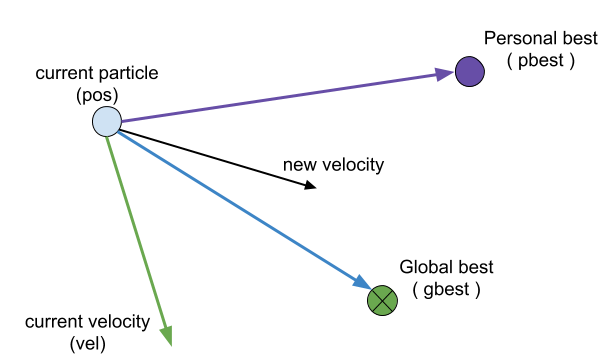
\includegraphics[width=4.0in]{_img/img_PSO_overview.png}
\caption{PSO overview}
\end{figure*}

For the CPU implementation we followed this simple variation of the asynchronous PSO algorithm :

\begin{algorithm*}
    \caption{Particle Swarm Optimization - Asynchonous Serial Version}\label{alg:PSOcpu}
    \begin{algorithmic}[1]
        \State $\textbf{In}: \textit{objFunction, populationSize, w, $c_{1}$, $c_{2}$, k, dimensions, domain}$
        \State $\textbf{Out}: \textit{Solution optima } P_{g.cost}$
        \State $vMin = -k * ( domain.max - domain.min ) / 2.0$
        \State $vMax =  k * ( domain.max - domain.min ) / 2.0$
        \State $P_{g.pos} = \textit{zeros( dimensions )}$ \Comment{Position that gives best cost}
        \State $P_{g.cost} = Inf$ \Comment{Best cost so far}
        \\
        \State $Particles=\lbrace \rbrace$ \Comment{Empty array of particles}
        \For {$i=1$ {\bfseries to} $PopulationSize$} \Comment{Particles Initialization}
            \State $p = \textbf{Particle()}$
            \State $p.pos = \textbf{randUniform( domain )}$
            \State $p.vel = \textbf{zeros( dimensions )}$
            \State $p.cost = \textbf{objFunction( p.pos )}$
            \State $p.bestpos = p.pos$
            \State $p.bestcost = p.cost$
            \If {$p.cost \leq P_{g.cost}$}
                \State $P_{g.cost} = p.cost$
                \State $P_{g.pos} = p.pos$
            \EndIf
        \EndFor
        \\
        \While {$\textit{ !stopCondition() }$} \Comment{Optimization process}
            \For {$p$ {\bfseries in} $Particles$}
                \State $p.vel = w * p.vel + 
                                c_{1} * ( p.bestpos - p.pos ) + 
                                c_{2} * ( P_{g.pos} - p.pos )$ \Comment{Velocity update}
                \State $p.vel = \textbf{ClampVector}\textit{( p.vel, vMin, vMax )}$
                \State $p.pos = p.pos + p.vel$ \Comment{Position update}
                \State $p.pos = \textbf{ClipPosition}\textit{( p.pos, domain )}$
                \\
                \If {$p.cost \leq p.bestcost$}
                    \State $p.bestcost = p.cost$ \Comment{Update personal best}
                    \State $p.bestpos = p.pos$
                    \If {$p.cost \leq P_{g.cost}$}
                        \State $P_{g.cost} = p.cost$ \Comment{Update global best}
                        \State $P_{g.pos} = p.pos$
                    \EndIf
                \EndIf
            \EndFor
        \EndWhile
        \\
        \Return $P_{g.cost}$
    \end{algorithmic}
\end{algorithm*}

For the GPU implementation we followed the same variation of the PSO algorithm in a synchronous way, by making the comparison with the global best outside of the particles update loop :

\begin{algorithm*}
    \caption{Particle Swarm Optimization - Synchonous Parallel Gpu Version}\label{alg:PSOgpu}
    \begin{algorithmic}[1]
        \State $\textbf{In}: \textit{objFunction, populationSize, w, $c_{1}$, $c_{2}$, k, dimensions, domain}$
        \State $\textbf{Out}: \textit{Solution optima } P_{g.cost}$
        \State $vMin = -k * ( domain.max - domain.min ) / 2.0$
        \State $vMax =  k * ( domain.max - domain.min ) / 2.0$
        \State $P_{g.pos} = \textit{zeros( dimensions )}$ \Comment{Position that gives best cost}
        \State $P_{g.cost} = Inf$ \Comment{Best cost so far}
        \\
        \State $hostParticles = \lbrace \rbrace$
        \State $deviceParticles = \lbrace \rbrace$
        \State $\textbf{GpuCreateParticles}\textit{( hostParticles, deviceParticles, objFunction, populationSize, dimensions, domain )}$
        \State $\textbf{GpuInitParticles}\textit{( hostParticles, deviceParticles, objFunction )}$
        \\
        \While {$\textit{ !stopCondition() }$} \Comment{Optimization process}
            \State $\textbf{GpuUpdateParticles}\textit{( hostParticles, deviceParticles, w, $c_{1}$, $c_{2}$, k )}$s
            \For {$p$ {\bfseries in} $hostParticles$}
                \If {$p.cost \leq P_{g.cost}$}
                    \State $P_{g.cost} = p.cost$ \Comment{Update global best}
                    \State $P_{g.pos} = p.pos$
                \EndIf
            \EndFor
        \EndWhile
        \Return $P_{g.cost}$
    \end{algorithmic}
\end{algorithm*}

\begin{algorithm*}
    \caption{Particle Swarm Optimization - GpuUpdateParticles}\label{alg:PSOgpu_kernel_updateparticles}
    \begin{algorithmic}[1]
        \State $\textbf{In}: \textit{deviceParticles, coreIndx, w, $c_{1}$, $c_{2}$, k, $P_{g}$}$
        \State $p = \textbf{getDeviceParticle}\textit{( coreIndx )}$
        \State $p.vel = w * p.vel + 
                        c_{1} * ( p.bestpos - p.pos ) + 
                        c_{2} * ( P_{g.pos} - p.pos )$ \Comment{Velocity update}
        \State $p.vel = \textbf{ClampVector}\textit{( p.vel, vMin, vMax )}$
        \State $p.pos = p.pos + p.vel$ \Comment{Position update}
        \State $p.pos = \textbf{ClipPosition}\textit{( p.pos, domain )}$
        \\
        \If {$p.cost \leq p.bestcost$}
            \State $p.bestcost = p.cost$ \Comment{Update personal best}
            \State $p.bestpos = p.pos$
        \EndIf
    \end{algorithmic}
\end{algorithm*}

\begin{figure*}
\centering
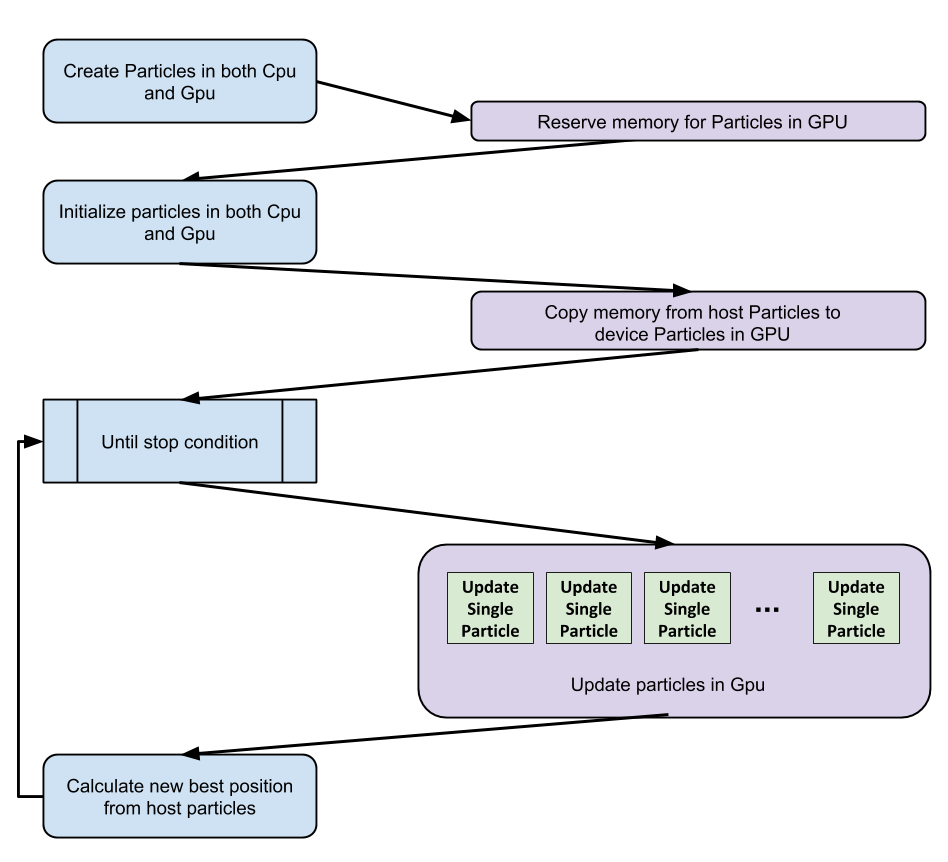
\includegraphics[width=4.0in]{_img/img_PSO_algorithm_gpu.png}
\caption{PSO algorithm in GPU}
\end{figure*}

\section{Results}

\begin{figure*}
\centering
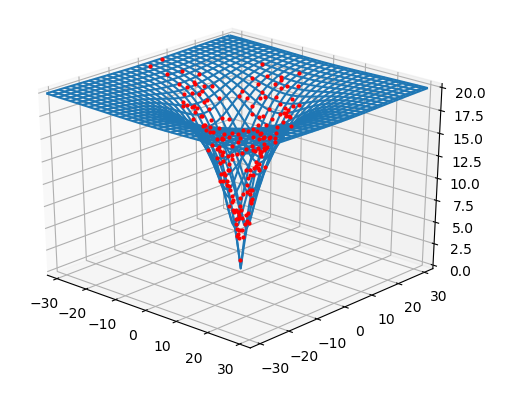
\includegraphics[width=3.0in]{_img/img_PSO_test_2d_ackley_3dview.png}
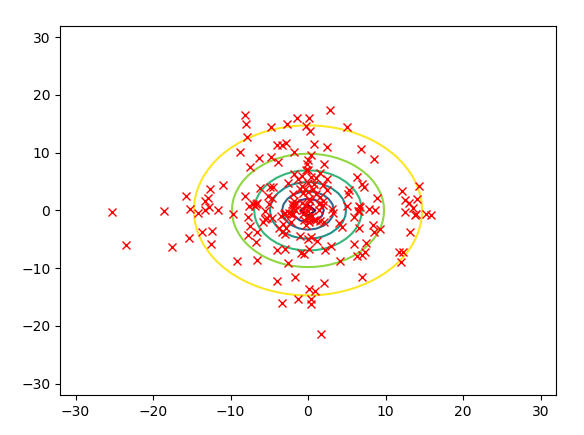
\includegraphics[width=3.0in]{_img/img_PSO_test_2d_ackley_contours.png}
\caption{PSO overview}
\end{figure*}

\begin{figure*}
\centering
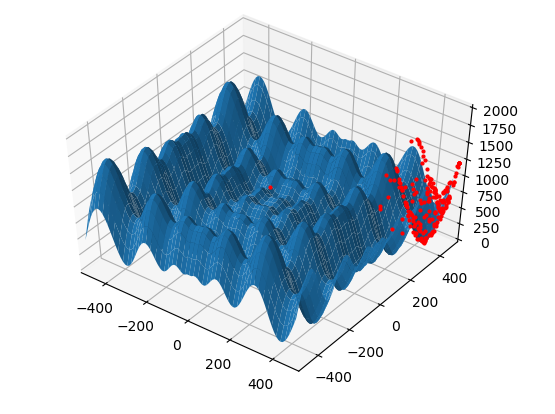
\includegraphics[width=3.0in]{_img/img_PSO_test_2d_schwefel_3dview.png}
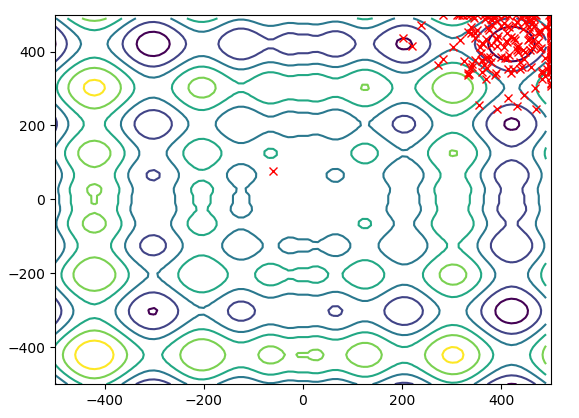
\includegraphics[width=3.0in]{_img/img_PSO_test_2d_schwefel_contours.png}
\caption{PSO overview}
\end{figure*}

\begin{figure*}
\centering
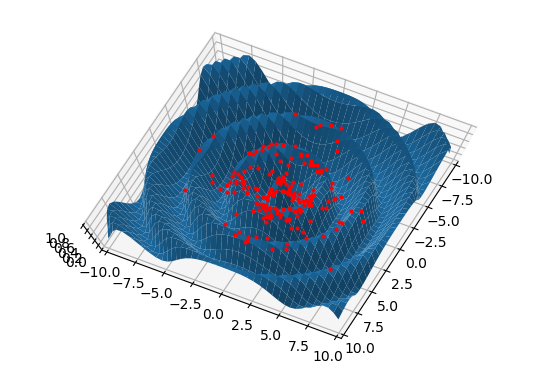
\includegraphics[width=3.0in]{_img/img_PSO_test_2d_schafferfcn6_3dview.png}
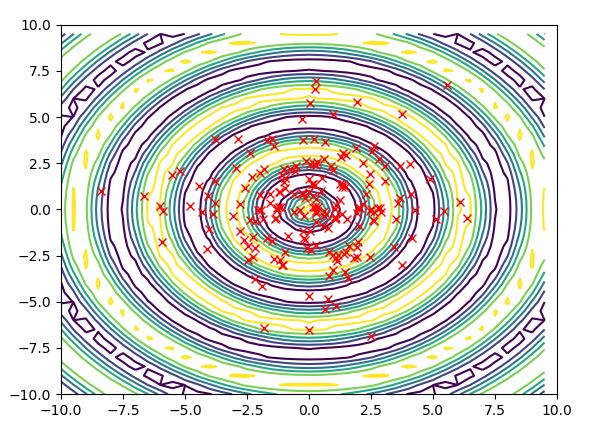
\includegraphics[width=3.0in]{_img/img_PSO_test_2d_schafferfcn6_contours.png}
\caption{PSO overview}
\end{figure*}

\section{Conclusions and Future improvements}


\IEEEtriggeratref{8}

% references section
\begin{thebibliography}{1}

\bibitem{Kennedy1995}
  James Kennedy and Russell Eberhart. \\
  \textit{Particle Swarm Optimization.} - 1995
\\
\bibitem{Garnier2007}
  Simon Garnier, Jacques Gautrais, Guy Theraulaz\\
  \textit{The biological principles of swarm intelligence.} - 2007
\\
\bibitem{delValle2008}
  Yamille del Valle, Ganesh Kumar, Salman Mohagheghi, Jean Hernandez, Ronald Harley\\
  \textit{Particle Swarm Optimization: Basic Concepts, Variants and Applications in Power Systems.} - 2008
\\
\bibitem{CameraCalibration1}
  Zhengyou Zhang \\
  \textit{A Flexible New Technique for Camera Calibration.} - 2000
\\
\bibitem{IntegralImageThresholding}
  Derek Bradley, Gerhard Roth \\
  \textit{Adaptive Thresholding Using the Integral Image.} - 2011

\end{thebibliography}


\end{document}
